% Use xelatex to generate pdf file of this presentation

\documentclass[xcolor=table]{beamer}
\usepackage{roboto}
\usepackage[russian]{babel}
\usetheme{Copenhagen}

% Simple way to put a code listing to the slide
\usepackage{listings}

% Tabular-specific packages
\usepackage{makecell}
\usepackage{tabu, booktabs}

\usepackage[symbol*]{footmisc}
\setfnsymbol{wiley}

\usepackage{tikz}
\usepackage{graphicx}
  \logo{
\includegraphics[scale=0.1]{pics/PostgresPro_logo}}
%Information to be included in the title page:
\title{pg\_index\_stats}
\subtitle{manage\ extended\ statistics\ automatically}
\author{\underline{Lepikhov A.}, Rybakina A.}
\institute{Postgres Professional}
%\titlegraphic{\includegraphics[scale=0.05]{project_url}}
\date{2024}

% Add page numbers in footnote
\expandafter\def\expandafter\insertshorttitle\expandafter{%
  \insertshorttitle\hfill%
  \insertframenumber\,/\,\inserttotalframenumber}

% Custom commands
\newcommand{\tbltext}[1]{\ttfamily\footnotesize#1}

% Custom colours: https://latexcolor.com
\definecolor{armygreen}{rgb}{0.29, 0.33, 0.13}
\definecolor{darkgreen}{rgb}{0.0, 0.5, 0.0}
\definecolor{lightlightgray}{gray}{0.9}

% Default listing format
\lstset{language=sql, frame=none, tabsize=2, identifierstyle=\color{black},
  showspaces=false, showtabs=false, showstringspaces=false,
  columns=fullflexible, % Restore default spaces between letters
  basicstyle=\rmfamily\scriptsize,
  stringstyle=\color{purple},
  keywordstyle=\bfseries\color{green!40!black},
  numberstyle=\tiny\color{gray}}

% -----------------------------

\begin{document}

% %%%%%%%%%%%%%%%%%%%%%%%%%%%%%%%%%%%%%%%%%%%%%%%%%%%%%%%%%%%%%%%%%%%%%%%%%%%%%%
%
% Title
%
% %%%%%%%%%%%%%%%%%%%%%%%%%%%%%%%%%%%%%%%%%%%%%%%%%%%%%%%%%%%%%%%%%%%%%%%%%%%%%%
\begin{frame}
\titlepage
   \tikz [remember picture,overlay]
    \node at
        ([yshift=2.0cm, xshift=-4.8cm]current page.center) 
        {
\includegraphics[scale=0.05]{pics/project_logo}};

\end{frame}

% My name is Andrei. Today, I want to spend this time talking about extending statistics and an extension we created to nudge improvement of PostgreSQL estimation techniques. Extended statistics dedicated to searching of correlations between columns in the table and predicting cardinality more accurately. Or, in other words, the size of the data returned by the table scan operator. It was introduced in the PG12, but since then, it has been used quite rarely because of some questions, like over which set of columns we should create these statistics. Or how to control the overhead of these statistics calculations. Because it is a costly procedure, of course.
% With a flow of performance reports related to the accuracy of optimizer predictions, we designed an extension that manages extended statistics creation/modification/removal. As a rationale of statistics management, we have chosen indexes. I'm going to explain how it works, the reasons for it, and usage examples.


% %%%%%%%%%%%%%%%%%%%%%%%%%%%%%%%%%%%%%%%%%%%%%%%%%%%%%%%%%%%%%%%%%%%%%%%%%%%%%%
%
% About me
%
% %%%%%%%%%%%%%%%%%%%%%%%%%%%%%%%%%%%%%%%%%%%%%%%%%%%%%%%%%%%%%%%%%%%%%%%%%%%%%%
\begin{frame}[fragile]\frametitle{Self Introduction}
\begin{columns}\begin{column}{0.6\textwidth}
\begin{itemize}
  \item Core Developer in Postgres Professional since 2017.
  \item Contributing to the PostgreSQL project since 2017:\\ \textit{Self-Join Elimination, GROUP-BY optimisation, OR <-> ANY transformation}.
  \item Ph.D. in Computer Sciences (Distributed Databases), MSU, 2008.
  \item Designed extensions: AQO, sr\_plan, pg\_index\_stats ...
\end{itemize}
\end{column}
\begin{column}{0.4\textwidth}
  \includegraphics[scale=0.05]{pics/selfie}
\end{column}\end{columns}
\end{frame}

% Because I am giving a speech for the first time in Asia, Let me tell you about myself shortly.
%I live in Thailand. I have been contributing to PostgreSQL since 2017. I am a core developer at Postgres Professional company. Most of my reviews and commits are dedicated to optimization issues. This year, two of my features were committed: Self-Join Removal and group-by optimization.
%I'm a Ph.D. Candidate in distributed databases, awarded in 2009. My most popular projects, which you would know, are Multimaster, Shardman, Adaptive Query Optimizer, and Plan Freezing. Previously, I attempted to resolve optimization issues with a query-driven approach. Nowadays, having experience of the limitations of the query-driven approach in PG, I'm attempting to resolve the planning issues with a data-driven approach, elaborating on statistics.
% KEY IDEA: data-driven approach can resolve weak points of query-driven approach.

% %%%%%%%%%%%%%%%%%%%%%%%%%%%%%%%%%%%%%%%%%%%%%%%%%%%%%%%%%%%%%%%%%%%%%%%%%%%%%%
%
% Extended Statistics short introduction
%
% %%%%%%%%%%%%%%%%%%%%%%%%%%%%%%%%%%%%%%%%%%%%%%%%%%%%%%%%%%%%%%%%%%%%%%%%%%%%%%

\begin{frame}[fragile]\frametitle{Extended Statistics}
\vskip0pt plus 1filll
CREATE STATISTICS ON x1,x2,x3,x4 FROM tablename;
\vspace{10pt}
\begin{itemize}
  \item \textbf{MCV} - \textbf{M}ost \textbf{C}ommon \textbf{V}alues on composite value  of (x1,x2,x3).
  \item \textbf{ndistinct} - number of distinct values on all combinations of columns: (x1,x2),(x1,x3),(x1,x2,x3)...
  \item \textbf{dependencies} - functional dependencies between combinations of columns: x1->x2, (x1,x2)->x3,...
\end{itemize}
\vskip0pt plus 1filll
\begin{columns}\begin{column}{0.03\textwidth}

\includegraphics[scale=0.1]{pics/vondra_extstat}
\end{column}\begin{column}{0.8\textwidth}
\textit{Vondra. T. CREATE STATISTICS improvements,\\ PGConf.DE 2022}
\end{column}\end{columns}
\end{frame}
%I want to explain the extended statistic a bit to ensure we are on the same page. The best description of that feature can be found in Tomas Vondra's recent presentation (see link below). He is the leading developer of this feature. You can find it by following the link in the QR code.
%This type of statistic is designed to provide information about the joint distribution of a set of columns or expressions. At the top of the slide you can see an example of its definition. Right now extended statistics can be built upon one table involving some set of columns or expressions.
%These statistics are still not extensible and include three types of data: number of distinct values, most common values and dependency factor.
%The number of distinct values is calculated for all possible combinations of the defining columns. The MCV is a collection of the most frequent values, and dependency shows us the factor of dependency between any possible combination of columns in the set of columns. 

\begin{frame}[fragile]\frametitle{Laboriousness of Extended Statistics}
\begin{itemize}
  \item \textbf{MCV} - two arrays: values[] and frequences[].
  \item \textbf{ndistinct} - 1 integer for each of $2^n - (n+1)$ combinations
  \item \textbf{dependencies} - 1 float value for each of combinations
\end{itemize}
\vspace{20pt}
\begin{center}
\begin{tabular}{|l|c|c|c|c|c|}
\hline
columns: & 2 & 3 & 4 & ... & 8 \\
\hline
distinct combinations: & 1 & 4 & 11 & ... & 247 \\
\hline
dependency combinations: & 2 & 9 & 28 & ... & 1016 \\
\hline
\end{tabular}
\end{center}
\end{frame}
% Let's see the complexity of maintaining such statistics in actual state.
% MCV is an array of data values and another one for their frequences. Here frequences are fixed-length real values. But data in the column, especially composite one can be lengthy and add overhead on detoasting.
% ndistinct is just one number and don't add a lot of overhead on reading and writing from the catalog. But the number of combinations are growing quickly with the number of columns involved. Here you can see exact numbers of such combinations. With 8 columns we must calculate it for 247 combinations during analysis.
% The same thing with dependencies. And even worse - for 8 columns we must generate 1016 combinations. It may be really expensive.
% Taking all above facts into account I think we should separate ANALYZE of plain and extended statistics somehow. Or, at least, add a parameter to the analyse command.
% KEY IDEA: separation from plain statistics and be careful about that.

% %%%%%%%%%%%%%%%%%%%%%%%%%%%%%%%%%%%%%%%%%%%%%%%%%%%%%%%%%%%%%%%%%%%%%%%%%%%%%%
%
% Example: how it works
%
% %%%%%%%%%%%%%%%%%%%%%%%%%%%%%%%%%%%%%%%%%%%%%%%%%%%%%%%%%%%%%%%%%%%%%%%%%%%%%%

\begin{frame}[fragile]\frametitle{Quick start}
\begin{lstlisting}[basicstyle=\footnotesize]
CREATE EXTENSION 'pg_index_stats';
CREATE TABLE test (x int,y int,z text);
CREATE INDEX ON test (x,y);
CREATE INDEX ON test (z,y);
\dX
\end{lstlisting}
\begin{lstlisting}[basicstyle=\tiny]
                         List of extended statistics
 Schema |     Name      |   Definition   | Ndistinct | Dependencies |   MCV   
--------+---------------+----------------+-----------+--------------+---------
 public | test_x_y_stat | x, y FROM test | defined   | defined      | defined
 public | test_z_y_stat | y, z FROM test | defined   | defined      | defined
\end{lstlisting}
\end{frame}
% MONOSPACE font here???
% To reduce DBA's headache we tried to introduce a module which must approach two issues: when to create and delete statistics, remove it and how to reduce overhead. Let me show you with example, how the extension address this issue. Here you can see a sequence of commands: at first, we create the extension. Second - create table and some indexes. Immediately after that, if you check extended statistics in the database you will see two new statistics created according to the definition of indexes. To reduce the risk of overhead we limit number of columns in auto-generated statistics and disallow duplicates. But we see a room for improvements here around compactifying statistics.

\begin{frame}[fragile]\frametitle{Quick start - II}
\begin{lstlisting}[basicstyle=\footnotesize]
DROP INDEX test_x_y_idx;
\end{lstlisting}
\begin{lstlisting}[basicstyle=\tiny]
                         List of extended statistics
 Schema |     Name      |   Definition   | Ndistinct | Dependencies |   MCV   
--------+---------------+----------------+-----------+--------------+---------
 public | test_z_y_stat | y, z FROM test | defined   | defined      | defined
\end{lstlisting}
\begin{lstlisting}[basicstyle=\footnotesize]
SELECT stxname,obj_description(oid, 'pg_statistic_ext')
FROM (SELECT oid,stxname FROM pg_statistic_ext);
\end{lstlisting}
\begin{lstlisting}[basicstyle=\tiny]
    stxname    |             obj_description              
---------------+------------------------------------------
 test_z_y_stat | pg_index_stats - multivariate statistics
\end{lstlisting}
\end{frame}
% Auto-generated statistics dependent on the extension and parent index. So,
% If you delete one of the indexes, after committing this operation, you will find only one statistic survived. Deleting the extension removes all auto-generated statistics if you don't change their dependencies in the system catalogue manually.
% Also, auto-generated statistics have some specific sign - it is a comment assigned for each such object: you can just use standard object description function to identify such statistics for some reasons - for example, to script your logic.
% KEY IDEA: complexity is managed by the index policy.

\begin{frame}[fragile]\frametitle{GUCs \& Funcs}
\begin{itemize}
  \item \textit{mode} - disabled | all | univariate | multivariate
  \item \textit{columns\_limit}
  \item \textit{pg\_index\_stats\_build(relname, mode)}
  \item \textit{pg\_index\_stats\_rebuild()}
  \item \textit{pg\_index\_stats\_remove()}
\end{itemize}
\end{frame}
% Also, the extension provides a few parameters related to the limitations and scope of the extension. We invented them because we quickly found that in real life, it could be harmful if someone creates an index containing 5-10 columns. And some people do that. No idea why.
% Moreover, you have functions to manually delete all such stats or rebuild them over all tables in the database or just over one heap table. 

\begin{frame}[fragile]\frametitle{Short Tech Dive}
Two-step process:
\begin{itemize}
  \item Object Access Hook - gather candidate OIDs 
  \item Utility Hook - create extended statistics after a successful utility statement
\end{itemize}
Set dependency of auto-generated statistics on the extension and index relation.\\
Add specific description for auto-generated statistics
\end{frame}
% A bit of tech details that can be useful for DBA and developers. We realised that it is challenging and not native for Postgres architecture to create a database object while creating another index object. Here, I talk about index and extension statistics built upon its definition. So, the procedure is divided into two steps:
% - Object creation. Here, we identify the creation of a table. You can't differentiate between plain tables, foreign tables, indexes, etc. We just save OID inside the extension.
% - Second step - is an end of utility operation. Here, we can already see the object have created, its type and name, and we can build extended statistics if this object is an appropriate index.
% And that's almost all about the extension. It's something like a TikTok-style speech. In the rest of the talk, I would like to explain why we have done it and how it works.

% %%%%%%%%%%%%%%%%%%%%%%%%%%%%%%%%%%%%%%%%%%%%%%%%%%%%%%%%%%%%%%%%%%%%%%%%%%%%%%
%
% Origins: why this problem emerging now?
%
% %%%%%%%%%%%%%%%%%%%%%%%%%%%%%%%%%%%%%%%%%%%%%%%%%%%%%%%%%%%%%%%%%%%%%%%%%%%%%%

\begin{frame}[fragile]\frametitle{Query auto-generation frameworks}
\begin{center}
	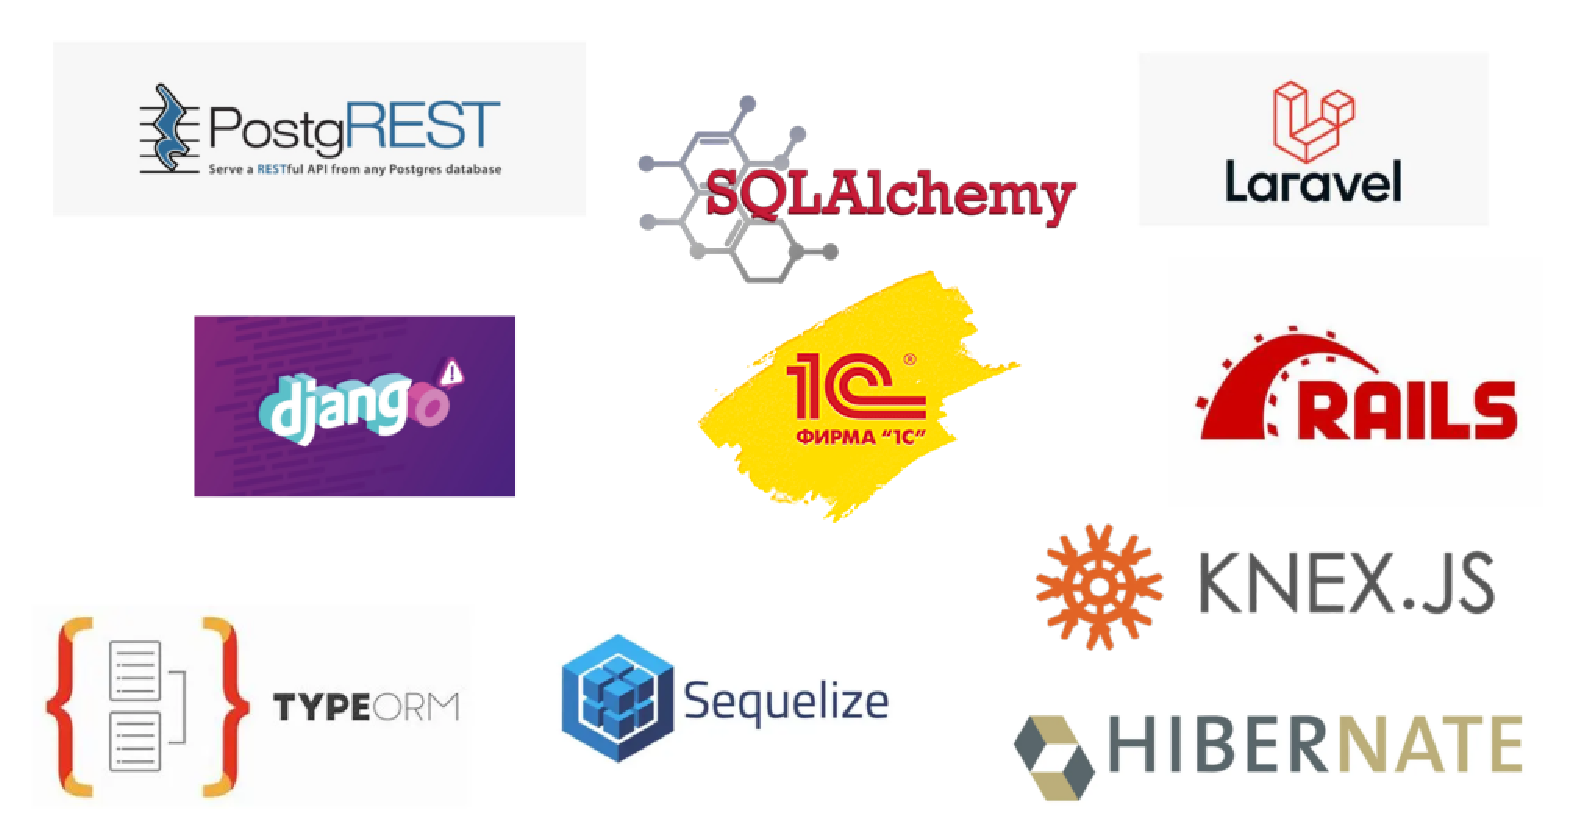
\includegraphics[scale=0.4]{pics/orms}
\end{center}
\end{frame}
% The main reason for this work is current high flow of queries, containing not-optimized list of filters or join clauses. The source of the problem are frameworks, like ORMs or restful api. They can generate quite complex queries and Postgres with assumption of uniform distribution everywhere makes quaint predictions very often.
% We are waiting that size of databases, managed with such frameworks in near future will steadily surge.

\begin{frame}[fragile]\frametitle{What is the reason?}
	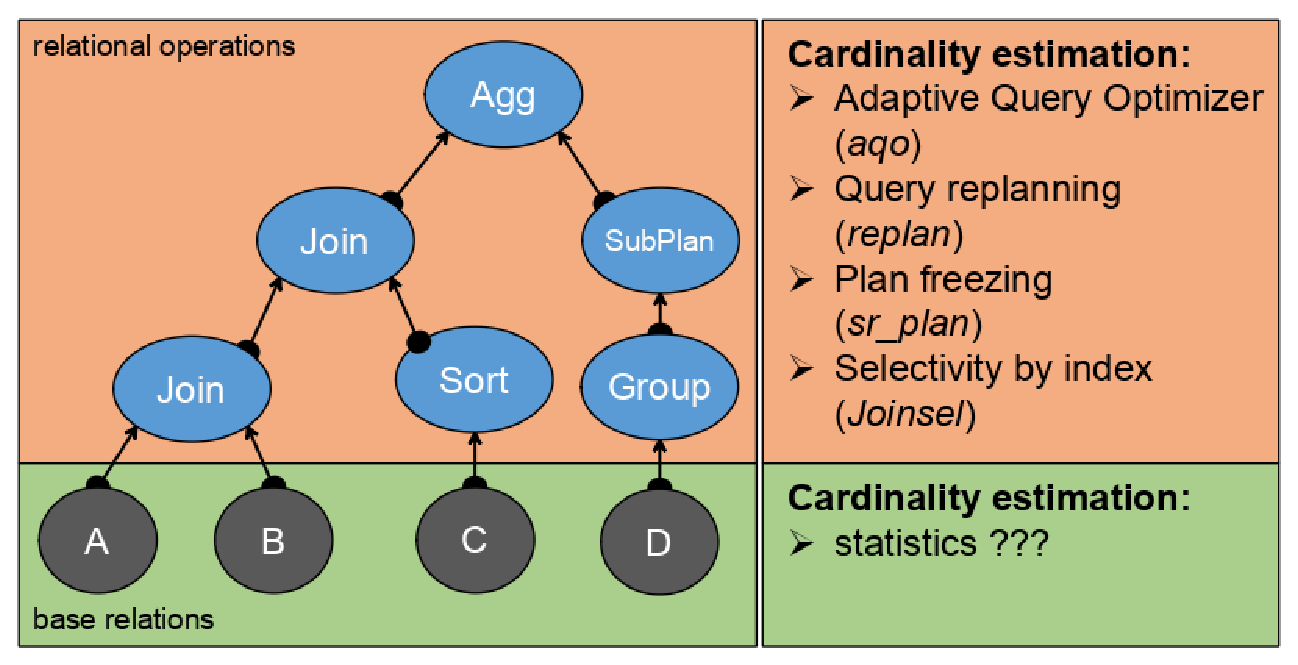
\includegraphics[scale=0.52]{pics/querytree}
\end{frame}
% Analysing and solving this problem we found, that on the query level of table scan we should use different techniques than on higher levels of JOINs, GROUP-BYs and other aggregates. Higher levels can be tolerant to estimation overhead, low level - not.
% For high levels we already have quite elaborate tools, but scan level estimation issue still may be resolved with only adequate statistics.

\begin{frame}[fragile]\frametitle{Redundant expressions}
\lstset{language=sql, frame=none, tabsize=2, identifierstyle=\color{black},
  backgroundcolor=\color{white},
  keywordstyle=\bfseries\color{green!40!black},showspaces=false, showtabs=false, showstringspaces=false}
\begin{center}
\begin{tabular}{|l|c|c|}
	\hline
	% Header
	\multicolumn{1}{|c|}{Query} & Planned rows & Actual rows \\
	\hline
\begin{lstlisting}[basicstyle=\footnotesize]
SELECT * FROM power_plants
WHERE
  country = 'RUS';
\end{lstlisting}
& \cellcolor{green}544 & \cellcolor{green}544 \\
	\hline
\begin{lstlisting}[basicstyle=\footnotesize]
SELECT * FROM power_plants
WHERE
  country = 'RUS' AND
  country_long = 'Russia';
\end{lstlisting}
& \cellcolor{red}8 & \cellcolor{green}544 \\
	\hline
\end{tabular}
\footnotetext{

\includegraphics[scale=0.4]{pics/GPPD-copyright}
}
\end{center}
\end{frame}
% Here you can see some trivial demonstration of the problem. I got database of power plants, freely accessible online. You can download it with the link provided at the bottom of the slide. This databsase contains only one table with multiple columns. Large data but not so much different values in each column quite typical case for our clients.
% Here we have only plain statistics, independent for each column.
% Querying database with country abbreviation only we have precise prediction. But adding into that query full name of the country we see huge underestimation. It is just because DBMS doesn't know about correlation between these two columns: Each country has unique abbreviation and full name. It may be stupid query, but with ORMs in the middle we see such queries frequently enough. So, my question is...

% %%%%%%%%%%%%%%%%%%%%%%%%%%%%%%%%%%%%%%%%%%%%%%%%%%%%%
%
% The main question that should be explained.
%
% %%%%%%%%%%%%%%%%%%%%%%%%%%%%%%%%%%%%%%%%%%%%%%%%%%%%%
\begin{frame}[fragile]\frametitle{The question}
\begin{quote}
Why can database systems, which manage all the data, not analyse it and find at least in-table dependencies and interconnections?
\end{quote}
\end{frame}
% DBMSes have whole set of data and information about constraints. Why, having also information about incoming queries they shouldn't have analyzed hidden correlations in data. In our opinion, having growing practice of automatization and also sustainability aspects, next step in the evolution of DBMSes should address this question in some way.
% This work - is a small step in that direction.

% %%%%%%%%%%%%%%%%%%%%%%%%%%%%%%%%%%%%%%%%%%%%%%%%%%%%%
%
% Rationale for the usage of indexes. An example.
%
% %%%%%%%%%%%%%%%%%%%%%%%%%%%%%%%%%%%%%%%%%%%%%%%%%%%%%
\begin{frame}[fragile]\frametitle{Why indexes?}
\begin{lstlisting}[basicstyle=\footnotesize]
Table "Parcels":
Indexes:
    "parcel_pkey" PRIMARY KEY, btree (id)
    "parcel_parcel_id" btree (parcel_id)
    "parcel_id_prik" btree (parcel_id, prik)
    "parcel_id_sn_pol" btree (parcel_id, sn_pol)
    "parcel_par_begin" btree (parcel_id, prik_begin_period)
    "parcel_par_patient" btree (parcel_id, patient_id)
    "parcel_par_recid" btree (parcel_id, recid)
    "parcel_per_prik" btree (period, prik)
\end{lstlisting}
\end{frame}
% Next question: why we have chasen indexes as a basis of our method. Looking into the common user practices we see, that the index usually is a template for most frequent or most important queries. btree indexes dependent on order of columns and users also frequently generate indexes on different orders of columns, trying to use it in the query. So, we have a big chance to get a query with filter over such specific set of columns, coming in such specific order. Covering these columns and these orders with extended statistics is a good strategy. Looking into this example of index coverage over a table you can understand, that we should inevitably stuck into the problem of compactifying the stats.

% %%%%%%%%%%%%%%%%%%%%%%%%%%%%%%%%%%%%%%%%%%%%%%%%%%%%%
%
% How extended statistics helps
%
% %%%%%%%%%%%%%%%%%%%%%%%%%%%%%%%%%%%%%%%%%%%%%%%%%%%%%
\begin{frame}[fragile]\frametitle{Extended v/s Plain Statistics}
SELECT * FROM power\_plants WHERE ...
\begin{center}
\begin{tabular}{|l|c|c|c|}
	\hline
	% Header
	\multicolumn{1}{|c|}{\tbltext{Query}} & \tbltext{\makecell{Plain\\ stat}} & \tbltext{\makecell{Extended\\ stat}} & \tbltext{\makecell{Actual\\ rows}} \\
	\hline
\begin{lstlisting}
country = 'RUS';
\end{lstlisting}
& \cellcolor{green}544 & \cellcolor{green}545 & \cellcolor{green}544 \\
	\hline
\begin{lstlisting}
AND primary_fuel IN ('Solar')
\end{lstlisting}
& \cellcolor{darkgreen}166 & \cellcolor{green}57 & \cellcolor{green}57 \\
	\hline
\begin{lstlisting}
primary_fuel IN
  ('Solar', 'Biomass')
\end{lstlisting}
& \cellcolor{darkgreen}189 & \cellcolor{green}60 & \cellcolor{green}60 \\
	\hline
\begin{lstlisting}
primary_fuel IN
  ('Solar', 'Biomass', 'Coal')
\end{lstlisting}
& \cellcolor{darkgreen}225 & \cellcolor{green}156 & \cellcolor{green}156 \\
	\hline
\begin{lstlisting}
AND source = 'Wiki-Solar'
\end{lstlisting}
& \cellcolor{red}24 & \cellcolor{green}46 & \cellcolor{green}40 \\
	\hline
\begin{lstlisting}
AND longitude > 40.
AND longitude < 70.
\end{lstlisting}
& \cellcolor{red}1 & \cellcolor{red}1 & \cellcolor{green}33 \\
	\hline
\end{tabular}
\footnotetext{

\includegraphics[scale=0.4]{pics/GPPD-copyright}
}
\end{center}
\end{frame}
% On the next slide I show comparison between cardinality estimation of trivial scan, when we use plain statistics and extended one.
% Here we have the same table on energy plants as I described above. We step-by-step add clauses to the filter: country, type of fuel, source of data and coordinates. As you can see, plain statistics goes into underestimation because doesn't detect dependencies in data. Extended statistic works better and breaks only at the last step, when we select data by geographical position of the plant. Extended statistics doesn't work properly with inequalities because of its nature. Here can help only histogram, but we haven't had multidimensional histograms in the core so far.

% %%%%%%%%%%%%%%%%%%%%%%%%%%%%%%%%%%%%%%%%%%%%%%%%%%%%%
%
% Why do we need a multicolumn histogram
%
% %%%%%%%%%%%%%%%%%%%%%%%%%%%%%%%%%%%%%%%%%%%%%%%%%%%%%
\begin{frame}[fragile]\frametitle{Does multicolumn histogram make sense?}
In general - no. We need a multidimensional histogram. But it can make sense if we follow the definition of indexes ...
\vspace{10pt}
\begin{lstlisting}
SELECT * FROM power_plants
WHERE
  country = 'RUS' AND
  primary_fuel IN ('Solar', 'Biomass', 'Coal') AND
  AND source = 'Wiki-Solar' AND
  longitude > 40. AND longitude < 70.;
\end{lstlisting}
\begin{center}
	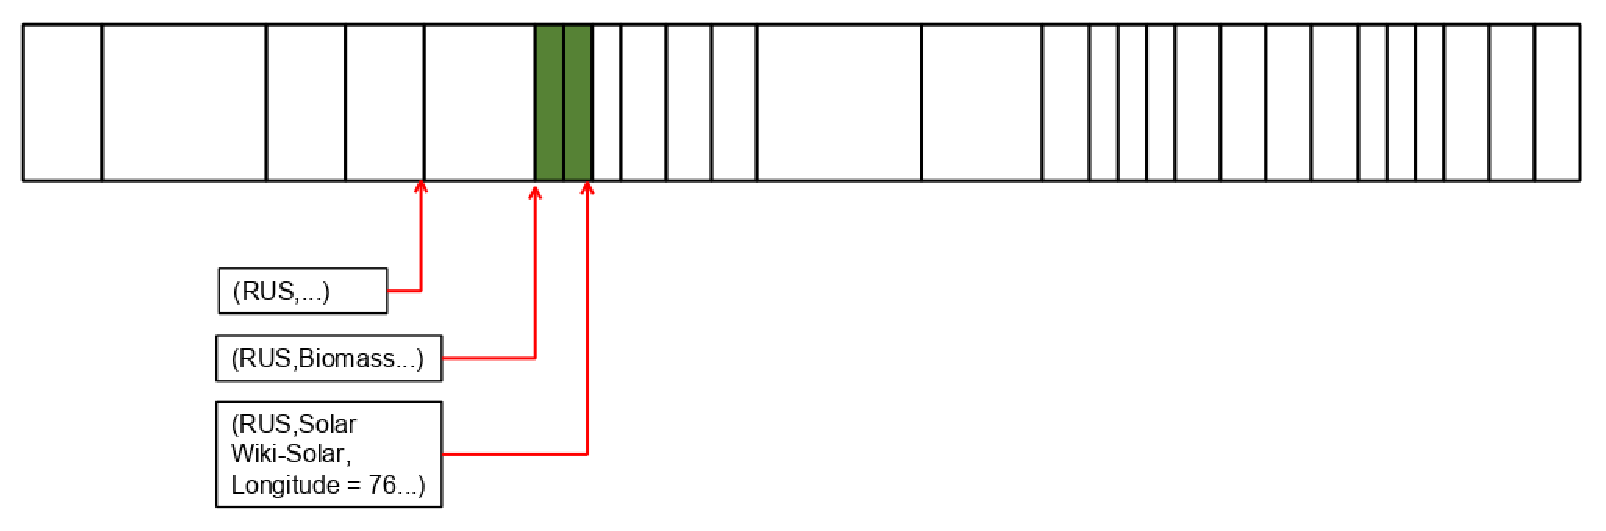
\includegraphics[scale=0.4]{pics/histogram}
\end{center}
\end{frame}
% The goods news here: because we establish our idea on indexes, we think we have predefined order of columns in the filter. In that case we can use trivial histogram, not a multidimensional histogram. And we invented a patch which generates such a histogram. Just looking for the top and bottom boundaries in the histogram it returns target bins where our data can be and allows avoid underestimation in all cases except stale statistics and help in the case of range queries where extended stat falls short.
% Of course, increasing number of columns in the composite type underlying the histogram we need increasingly more precise resolution of the histogram. And for small number of returning data it will not work precisely enough, but can help with big data sets.

% %%%%%%%%%%%%%%%%%%%%%%%%%%%%%%%%%%%%%%%%%%%%%%%%%%%%%
%
% Extended statistics v/s histogram
%
% %%%%%%%%%%%%%%%%%%%%%%%%%%%%%%%%%%%%%%%%%%%%%%%%%%%%%
\begin{frame}[fragile]\frametitle{Multicolumn histogram advantage}
SELECT * FROM power\_plants WHERE ...
\begin{center}
\begin{tabular}{|l|c|c|c|c|}
	\hline
	% Header
	\multicolumn{1}{|c|}{\tbltext{Query}} & \tbltext{\makecell{Plain\\ stat}} & \tbltext{\makecell{Extended\\ stat}} & \tbltext{Histogram} & \tbltext{\makecell{Actual\\ rows}} \\
	\hline
\begin{lstlisting}
country = 'RUS';
\end{lstlisting}
& \cellcolor{green}544 & \cellcolor{green}545 & \cellcolor{green}544 & \cellcolor{green}544 \\
	\hline
\begin{lstlisting}
AND primary_fuel IN ('Solar')
\end{lstlisting}
& \cellcolor{darkgreen}166 & \cellcolor{green}57 & \cellcolor{green}57 & \cellcolor{green}57 \\
	\hline
\begin{lstlisting}
primary_fuel IN
  ('Solar', 'Biomass')
\end{lstlisting}
& \cellcolor{darkgreen}189 & \cellcolor{green}60 & \cellcolor{green}60 & \cellcolor{green}60 \\
	\hline
\begin{lstlisting}
primary_fuel IN
  ('Solar', 'Biomass', 'Coal')
\end{lstlisting}
& \cellcolor{darkgreen}225 & \cellcolor{green}156 & \cellcolor{green}156 & \cellcolor{green}156 \\
	\hline
\begin{lstlisting}
AND source = 'Wiki-Solar'
\end{lstlisting}
& \cellcolor{red}24 & \cellcolor{green}46 & \cellcolor{green}42 & \cellcolor{green}40 \\
	\hline
\begin{lstlisting}
AND longitude > 40.
AND longitude < 70.
\end{lstlisting}
& \cellcolor{red}1 & \cellcolor{red}1 & \cellcolor{green}35 & \cellcolor{green}33 \\
	\hline
\end{tabular}
\footnotetext{

\includegraphics[scale=0.4]{pics/GPPD-copyright}
}
\end{center}
\end{frame}
% Here we continued the experiment with complex selection filter and utilized this patch with histogram to see how it can work. The same queries, the same steps of adding new clauses and one additional column for histogram selectivity as a right column of the table. As you can see, histogram follows the extended statistics. The reason here is low number of distinct values in each column. It is just a trick for demonstration. But, see the bottom row of this table, histogram allows postgres to make objective estimation of selectivity with inequality, catching the fact, that most of Russian power plants located in the deep north semisphere.
This experiment shows that we need at least additional statistics, may be histograms. And to add factual information and real user experience here we must develop small number of new hooks on clauses estimation and statistics generation. Because people don't like extensions with core patches.

% %%%%%%%%%%%%%%%%%%%%%%%%%%%%%%%%%%%%%%%%%%%%%%%%%%%%%
%
% Final frame
%
% %%%%%%%%%%%%%%%%%%%%%%%%%%%%%%%%%%%%%%%%%%%%%%%%%%%%%
\begin{frame}
\begin{center}
\begin{center}

\includegraphics[scale=0.1]{pics/project_logo}
\end{center}
\huge{Questions ?}
\end{center}
\vspace{10pt}
\begin{center}
\begin{tabular}{rl}
\makecell[c]{
\includegraphics[scale=0.1]{pics/extensionlink}} & \tbltext{\makecell[l]{The pg\_index\_stats extension\\ github link}} \\
\makecell[c]{
\includegraphics[scale=0.1]{pics/pgpro}} & \tbltext{\makecell[l]{Postgres Professional LLC\\ The Russian Postgres Company}} \\
\end{tabular}
\end{center}
\end{frame}

\end{document}
